\documentclass[a4paper,11pt]{article}
\usepackage[utf8]{inputenc}
\usepackage{lastpage}
\usepackage{fancyhdr}
\usepackage[english]{babel}
\usepackage[a4paper,margin=1in]{geometry}
\usepackage{multirow}
\usepackage[table,xcdraw]{xcolor}
\usepackage{array}
\usepackage{graphicx}
\usepackage{caption}
\usepackage{ctable}
\usepackage{listings}
\usepackage[T1]{fontenc}
\usepackage{bigfoot} % to allow verbatim in footnote
\usepackage[numbered,framed]{matlab-prettifier}
\usepackage{amsmath}


\newcolumntype{L}[1]{>{\raggedright\let\newline\\\arraybackslash\hspace{0pt}}m{#1}}
\newcolumntype{C}[1]{>{\centering\let\newline\\\arraybackslash\hspace{0pt}}m{#1}}
\newcolumntype{R}[1]{>{\raggedleft\let\newline\\\arraybackslash\hspace{0pt}}m{#1}}

\newcommand\tab[1][4mm]{\hspace*{#1}}


%-------------------------------------------------------------------------------
% HEADER & FOOTER
%-------------------------------------------------------------------------------

\pagestyle{fancy}
\fancyhf{}
\setlength\headheight{15pt}
\fancyhead[L]{ Imaging Lab 9 }
\fancyhead[R]{Student ID: 100633486}
\fancyfoot[R]{Page \thepage\ of \pageref{LastPage}}


%-------------------------------------------------------------------------------
% TITLE PAGE
%-------------------------------------------------------------------------------

\begin{document}

\title{
	\Huge \textbf {Contour-based Segmentation}
    \\ [0.2cm]
	\LARGE Imaging Lab 9 - May, 2017
    \\ [0.5cm]
    \hrule
}

\date{}

\author{
		\Large Kamyar Nazeri \\
		\large Student ID: 100633486 }

\maketitle
\newpage

\section*{Chan-Vese (CV) segmentation}
Image segmentation is the process of partitioning a digital image into multiple segments. Here we are using Deformable Models to do segmentation which is evolving a contour $\Gamma$ that snaps around objects. Chan-Vese Active Contours Model is an example of deformable model and its 2-phase model is:
\begin{align*}
\boldsymbol{\min \limits_{\Gamma}\ E_{CV}[\Gamma|f] = L(\Gamma) + \lambda_{in} \int\limits_{inside\ \Gamma}(f - c_{in})^2 d\vec{x} + \lambda_{out} \int\limits_{inside\ \Gamma}(f - c_{out})^2 d\vec{x}}
\end{align*}
Where $L(\Gamma)$ is the length of the curve and $c$ is the average gray value of $f$ in each region. By using The Heaviside Function, these equations become:
\begin{align*}
& \tab\tab L(\Gamma) = \int\limits_{\Omega} \Vert\nabla H(\phi)\Vert d\vec{x} = \int\limits_{\Omega} \delta(\phi) \Vert\nabla \phi \Vert d\vec{x} \\\\
& c_{in} = \frac{\int\limits_{\Omega} H(\phi)f d\vec{x}}{\int\limits_{\Omega} H(\phi) d\vec{x}} \tab\tab\tab\tab\tab
c_{out} = \frac{\int\limits_{\Omega} (1 - H(\phi))f d\vec{x}}{\int\limits_{\Omega} (1 - H(\phi)) d\vec{x}}
\end{align*}
By minimizing the steepest descent to evolve the PDE:
\begin{align*}
\frac{\partial \phi}{\partial t} = \delta(\phi) \bigg[ \nabla\cdot(\frac{\nabla\phi}{|\nabla\phi|}) -  \lambda_{in} (f - c_{in})^2 + \lambda_{out} (f - c_{out})^2 \bigg]
\end{align*}
Where $\delta(\phi)$ is the Dirac delta function, and we use a smooth approximation for it:
\begin{align*}
\delta_{\epsilon}(t) = \frac{\epsilon}{\pi(\epsilon^2 + t^2)}
\end{align*}
We initialize segmenting a test image using 1) a large circle in the center of the image and 2) a small circle around a user specified starting point. \\
To draw a large circle in the center of the image we use the following Matlab code:
\begin{lstlisting}[
    style=Matlab-editor,
    numbers=none,
    frame=none,
    xleftmargin=.2in
]
    [x,y] = meshgrid(1:n, 1:m);
    D = [(x - n/2).^2 + (y - m/2).^2 <= 100^2];
\end{lstlisting}
 \\
To allow the user to pick a starting point on the image, we use Matlab's \emph{ginput} function, locate point clicked by the user and draw a small circle around it:
\begin{lstlisting}[
    style=Matlab-editor,
    numbers=none,
    frame=none,
    xleftmargin=.2in
]
    imshow(uint8(f));
    P = ginput(1);
    [x,y] = meshgrid(1:n, 1:m);
    D = [(x - P(1)).^2 + (y - P(2)).^2 <= 3^2];
\end{lstlisting}
To prevent a sudden jump in the gradient of the level set, we use the signed distance smooth level set function using Matlab's $bwdist$ command:
\begin{lstlisting}[
    style=Matlab-editor,
    numbers=none,
    frame=none,
    xleftmargin=.2in
]
    u = bwdist(1-D) - bwdist(D);
    u = 0.1 * u;
\end{lstlisting}
Note that we scale the level set function down, to make our segmentation algorithm faster.

\newpage
\section*{Coding Chan-Vese Segmentation}
\emph{Listing 1} shows the Chan-Vese Segmentation applied on a grayscale image in Matlab, note that the initial level set function is specified by the user: \\
\begin{lstlisting}[caption={Chan-Vese Segmentation function for grayscale images in Matlab},captionpos=b,style=Matlab-editor]
function [u] = CVINT(f, init, lambda)
    % Chan-Vese segmentation algorithm using level sets

    %Parameters
    dt = 0.2;               % time step
    T = 100;                % stopping time
    a = 0.1;                % fudge factor
    e = 0.1;                % epsilon (Dirac function)
    [m,n] = size(f);        % image size
    f = double(f);          % convert to double
    u = init;

    for t = 0:dt:T
        % u_x = (u(x+1,y) - u(x-1,y)) / 2
        u_x = (u(:,[2:n,n]) - u(:,[1,1:n-1])) / 2;

        % u_y = (u(x,y+1) - u(x,y+1)) / 2
        u_y = (u([2:m,m],:) - u([1,1:m-1],:)) / 2;

        % u_xx = u(x+1,y) - 2u(x,y) + u(x-1,y)
        u_xx = u(:,[2:n,n]) - 2 * u + u(:,[1,1:n-1]);

        % u_yy = u(x,y+1) - 2u(x,y) + u(x,y-1)
        u_yy = u([2:m,m],:) - 2 * u + u([1,1:m-1],:);

        % u_xy = (u(x+1,y+1)+u(x-1,y-1)-u(x-1,y+1)-u(x+1,y-1))/4
        u_xy = (u([2:m, m],[2:n, n]) + u([1,1:m-1], [1,1:n-1]) -  u([2:m, m],[1, 1:n-1]) - u([1, 1:m-1],[2:n, n])) / 4;

        num = (u_xx.*u_y.^2)-2*(u_x.*u_z.*u_xy)+(u_yy.*u_x.^2);
        denom = (u_x.^2 + u_y.^2).^(3/2) + a;

        % The Dirac delta function, we use a smooth approximation
        drc = e ./(pi * (e^2 + u.^2));

        % the average gray value of f inside the region
        cin =  sum(sum(f .* [ u > 0 ])) / sum(sum([u > 0]));

        % the average gray value of f outside the region
        cout =  sum(sum(f .* [ u < 0 ])) / sum(sum([u <0 ]));

        pde = drc.*(num./denom-lambda*((f-cin).^2+(f-cout).^2));
        u = u + dt * pde;
    end
end


\end{lstlisting}

\newpage

\emph{Figure 1} shows segmenting a test image using a large circle in the center of the image:

\begin{figure}[!htb]
  \centering
  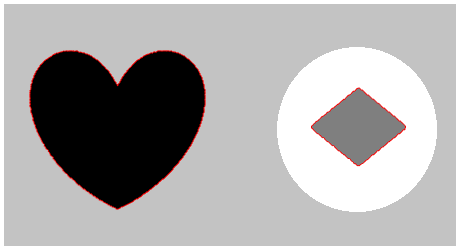
\includegraphics[width=8cm, height=4.3cm]{1.png}
  \caption{\small Chan-Vese Segmentation with a large circle in the center as the init level set function.}
\end{figure}

 \\
\emph{Figure 2} shows segmenting specific shapes in a test image by drawing a small circle around a user specified starting point as the init level set function:

\begin{figure}[!htb]
  \centering
  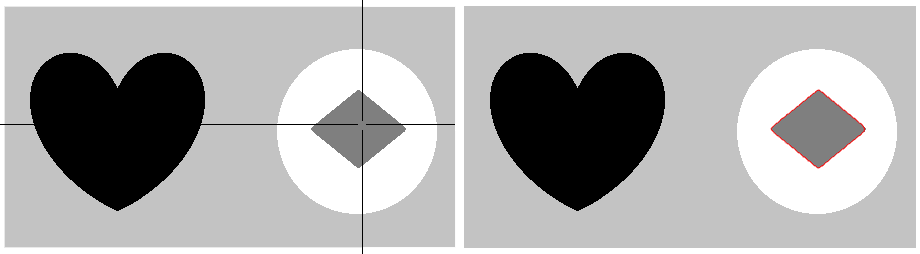
\includegraphics[width=16cm, height=4.42cm]{2.png}
\end{figure}

\begin{figure}[!htb]
  \centering
  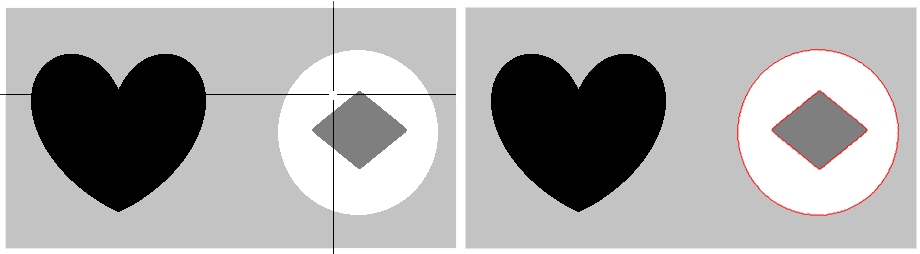
\includegraphics[width=16cm, height=4.42cm]{3.png}
\end{figure}

\begin{figure}[!htb]
  \centering
  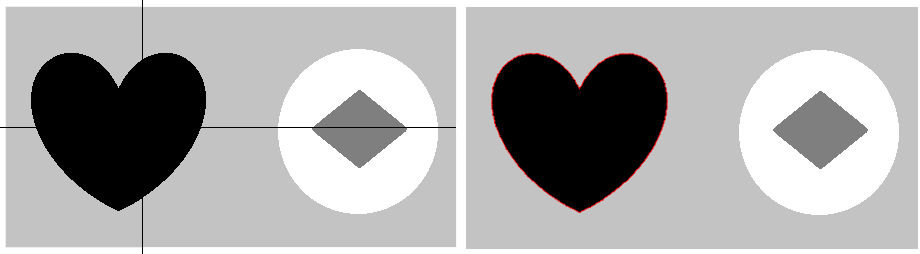
\includegraphics[width=16cm, height=4.42cm]{4.png}
  \caption{\small Chan-Vese Segmentation with a small circle around a user specified starting point as the init level set function.}
\end{figure}

\end{document}
